\documentclass[a4paper,11pt]{article}
\usepackage{jheppub}
\usepackage{url}
\RequirePackage{color,graphicx}
\usepackage{mathtools}
\usepackage{amsfonts}
\usepackage{amsthm}
\begingroup
    \makeatletter
    \@for\theoremstyle:=definition,remark,plain\do{%
        \expandafter\g@addto@macro\csname th@\theoremstyle\endcsname{%
            \addtolength\thm@preskip\parskip
            }%
        }
\endgroup
\usepackage{parskip}
\usepackage{pgfplots}
\pgfplotsset{compat=1.14}
\usepackage{tikz-cd}

\theoremstyle{definition}
\newtheorem*{defn}{Definition}
\newtheorem*{prop}{Proposition}
\newtheorem*{ex}{Example}
\newtheorem*{exs}{Examples}
\newtheorem*{thm}{Theorem}
\newtheorem*{lem}{Lemma}
\newtheorem*{cor}{Corollary}
\newtheorem*{rmks}{Remarks}

\DeclareMathOperator{\Int}{Int}
\DeclareMathOperator{\im}{im}

\newcommand\numberthis{\addtocounter{equation}{1}\tag{\theequation}}


\numberwithin{equation}{section}

\makeatletter
\def\@fpheader{
    %
}
\makeatother
\title{Statistics}

\author{Mathematical Tripos Part IB}
\affiliation{University of Cambridge}

\begin{document}
\maketitle
\flushbottom
\clearpage

Statistics is a set of principles and procedures for gaining and processing quantitative evidence in order to help us make judgements and decisions. This course focuses on formal \emph{statistical inference}, where we assume that we have some data generated from an unknown probability model, and aim to use the data to learn about certain properties of the underlying probability model.

In particular, we follow \emph{parametric inference}: we assume that a random variable $X$ follows a particular known family of distributions (e.g. Poisson) with unknown parameters. We then attempt to estimate the parameter from the data given.

Usually, the experiment is repeated several times, resulting in a collection of random variables $(X_1,...,X_n)$ which are i.i.d. with the same distribution as $X$. We then call the set $\mathbf{X}=(X_1,...,X_n)$ a \emph{simple random sample}, the data we have. Using the observed $\mathbf{X}=\mathbf{x}$, we can make inferences about the parameter $\theta$, such as
\begin{itemize}
    \item giving an estimate $\hat{\theta}(\mathbf{x})$ of the true value of $\theta$
    \item giving an interval estimate $(\hat{\theta}_1(\mathbf{x}),\hat{\theta}_2(\mathbf{x}))$ for $\theta$
    \item testing a hypothesis about $\theta$, e.g. $\theta=0$.
\end{itemize}

\hrulefill

\textbf{Estimation.}
Review of distribution and density functions, parametric families. Examples: binomial, Poisson, gamma. Suffciency, minimal suffciency, the Rao-Blackwell theorem. Maximum likelihood estimation. Confdence intervals. Use of prior distributions and Bayesian inference.

\textbf{Hypothesis testing.}
Simple examples of hypothesis testing, null and alternative hypothesis, critical region, size, power, type I and type II errors, Neyman-Pearson lemma. Signifcance level of outcome. Uniformly most powerful tests. Likelihood ratio, and use of generalised likelihood ratio to construct test statistics for composite hypotheses. Examples, including t-tests and F-tests. Relationship with confdence intervals. Goodness-of-fit tests and contingency tables.

\textbf{Linear models.}
Derivation and joint distribution of maximum likelihood estimators, least squares, Gauss-Markov theorem. Testing hypotheses, geometric interpretation. Examples, including simple linear regression and one-way analysis of variance. Use of software.

\hrulefill
\clearpage

\section{Estimation}
The aim of estimation is as follows: given i.i.d $X_1,...,X_n$ with known probability density/mass function $f_X(x;\theta)$, we want to estimate the unknown parameter $\theta$.

\begin{defn}[Statistic]
A \emph{statistic} is an estimate of $\theta$. It is a function $T$ of the data. Writing the data as $\mathbf{x}=(x_1,...,x_n)$, then our estimate is written as $\hat{\theta}=T(\mathbf{x})$. We call $T(\mathbf{X})$ the estimator of $\theta$, and the distribution of $T=T(\mathbf{X})$ the \emph{sampling distribution} of the statistic.
\end{defn}

Note that we adopt the convention where capital $\mathbf{X}$ denotes a random variable and $\mathbf{x}$ is an observed value. So $T(\mathbf{X})$ is a random variable whereas $T(\mathbf{x})$ is a particular value we obtain after experiments.

\begin{ex}
Let $X_1,...,X_n$ be i.i.d $N(\mu,1)$. A possible estimator for $\mu$ is 
\[
T(\mathbf{X})=\frac{1}{n}\sum_i X_i\,.
\]
Then for any particular observed sample $\mathbf{x}$, our estimate is
\[
T(\mathbf{x})=\frac{1}{n}\sum_i x_i\,.
\]
Now recall that in general if $X_i\sim N(\mu_i,\sigma_i^2)$, then $\sum X_i\sim N(\sum\mu_i,\sum\sigma_i^2)$, which can be proved by considering moment generating functions. So we have $T(\mathbf{X})\sim N(\mu,1/n)$.\footnote{By the Central Limit Theorem, even if $X_i$ were not normal, we still have approximately $T(\mathbf{X})\sim N(\mu,1/n)$ for large values of $n$, but here we get exactly the normal distribution for small values of $n$.}
\end{ex}

Our estimator of $\mu$ is a rather sensible estimator. We can always have less sensible estimators, such as $T(\mathbf{X})=X_1$, or even $T(\mathbf{X})=1$. To see how sensible an estimator is, we can look at its bias.

\begin{defn}[Bias]
Let $\hat{\theta}=T(\mathbf{X})$ be an estimator of $\theta$. Then the \emph{bias} of $\hat{\theta}$ is the difference between its expected value and true value,
\[
\text{bias}(\hat{\theta})=\mathbb{E}_\theta(\hat{\theta})-\theta\,.
\]

An estimator is \emph{unbiased} if it has no bias, i.e. $\mathbb{E}_\theta(\hat{\theta}))=0$.
\end{defn}

Note that the subscript in $\mathbb{E}_\theta$ does not represent the random variable, but the parameter we want to estimate. This is inconsistent with the use for, say, the probability mass function.

To find $\mathbb{E}_\theta(T)$, we can either find the distribution of $T$ and find its expected value, or evaluate $T$ as a function of $X$ directly, and find its expected value.

\begin{ex}
In the above example, $\mathbb{E}_\mu(T)=\mu$. So $T$ is unbiased for $\mu$.
\end{ex}

\subsection{Mean squared error}
Given an estimator, we want to know how good the estimator is. It turns out that the concept of bias is generally not a good measure of how good an estimator is. This can be illustrated by the following example:

Suppose we do 1000 random trials $X_1,...,X_{1000}$, and pick our estimator as $T(\mathbf{X})=X_1$. This is an unbiased estimator, but makes no use of our other 999 trials. On the other hand, $T'(\mathbf{X})=0.01+\frac{1}{1000}\sum X_i$ is biased (with a bias of 0.01), but is in general much more trustworthy than $T$. 

\begin{defn}
The \emph{mean squared error} of an estimator $\hat{\theta}$ is $\mathbb{E}_\theta[(\hat{\theta}-\theta)^2]$.

Sometimes we use the root mean squared error, which is the square root of the mean squared error.
\end{defn}

We can express the mean squared error in terms of the variance and bias:
\begin{align*}
\mathbb{E}_\theta[(\hat{\theta}-\theta)^2]&=\mathbb{E}_\theta[(\hat{\theta}-\mathbb{E}_\theta(\hat{\theta})+\mathbb{E}_\theta(\hat{\theta})-\theta)^2]\\
&=\mathbb{E}_\theta[(\hat{\theta}-\mathbb{E}_\theta(\hat{\theta})^2]+(\mathbb{E}_\theta(\hat{\theta})-\theta)^2+2(\mathbb{E}_\theta(\hat{\theta})-\theta)\mathbb{E}_\theta[\hat{\theta}-\mathbb{E}_\theta(\hat{\theta})]\\
&=\text{var}(\hat{\theta})+\text{bias}^2(\hat{\theta})\,.
\end{align*}

If we are aiming for a low mean squared error, it can sometimes be preferable to have a biased estimator with a lower variance. This is known as the ``bias-variance trade-off".

\begin{ex}
Suppose $X\sim\text{binomial}(n,\theta)$. The standard estimator is $T_U=X/n$, which is unbiased. This has variance
\[
\text{var}_\theta(T_U)=\frac{\text{var}_\theta(X)}{n^2}=\frac{\theta(1-\theta)}{n}\,,
\]
so the mean squared error of the usual estimator is
\[
\text{mse}(T_U)=\text{var}_\theta(T_U)+\text{bias}^2(T_U)=\frac{\theta(1-\theta)}{n}\,.
\]
Now consider an alternative estimator
\[
T_B=\frac{X+1}{n+2}=w\frac{X}{n}+(1-w)\frac{1}{2}\,,
\]
where $w=n/(n+2)$. This can be interpreted as a weighted average (by the sample size) of the sample mean and $1/2$. This gives
\[
\mathbb{E}_\theta(T_B)-\theta=\frac{n\theta+1}{n+2}-\theta=(1-w)\left(\frac{1}{2}-\theta\right)\,,
\]
so it is biased. The variance is given by
\[
\text{var}_\theta(T_B)=\frac{\text{var}_\theta(X)}{(n+2)^2}=w^2\frac{\theta(1-\theta)}{n}\,,
\]
and so the mean squared error is
\[
\text{mse}(T_B)=\text{var}_\theta(T_B)+\text{bias}^2(T_B)=w^2\frac{\theta(1-\theta)}{n}+(1-w)^2\left(\frac{1}{2}-\theta\right)\,.
\]
For $n=10$, observe the plot below.
\begin{figure}[h]
    \centering
    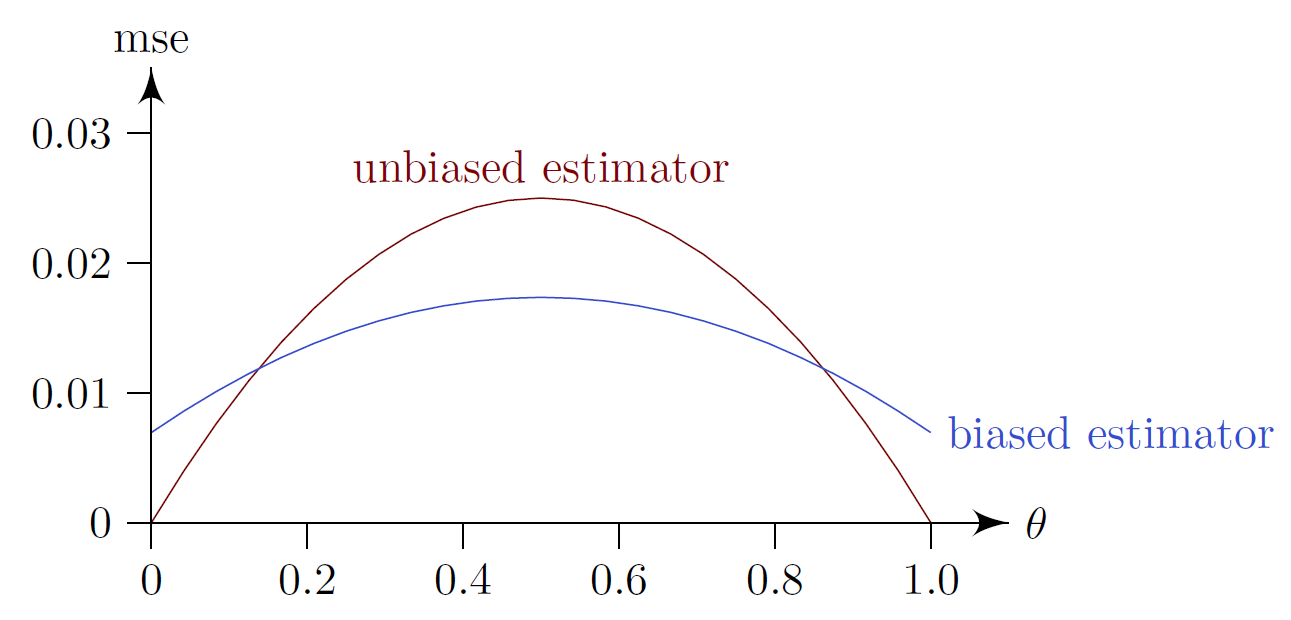
\includegraphics[width=0.7\textwidth]{estimator.PNG}
    \label{fig:estimator}
\end{figure}
We see that the biased estimator has a smaller MSE unless $\theta$ has extremal values. So sometimes biased estimators can give better mean squared errors.
\end{ex}

In fact, unbiased estimators can be complete nonsense.

\begin{ex}
Suppose $X\sim\text{Poisson}(\lambda)$, and that we want to estimate $\theta=(P(X=0))^2=e^{-2\lambda}$. Then any unbiased estimator $T(X)$ must satisfy $\mathbb{E}_\theta(T(X))=\theta$, or equivalently
\[
E_\lambda(T(X))=e^{-\lambda}\sum_{x=0}^\infty T(x)\frac{\lambda^x}{x!}=e^{-2\lambda}\,.
\]

The only function that can satisfy this equation is $T(X)=(-1)^X$. Then the unbiased estimator would estimate $e^{-2\lambda}$ to be $1$ if $X$ is even, and $-1$ if $X$ odd, which clearly does not make sense.
\end{ex}

\subsection{Sufficiency}
Often, we do experiments just to find out the value of $\theta$. For example, we might want to estimate the proportion of the population that supports some political candidate. We are seldom interested in the data points themselves, and just want to know the big picture. This leads to the concept of \emph{sufficient statistic}. This is a statistic $T(X)$ that contains all information we have about $\theta$ in the sample.

\begin{ex}
Let $X_1,...,X_n$ be i.i.d $\text{Bernoulli}(\theta)$, so that $\mathbb{P}(X_i=1)=1-\mathbb{P(X)}=\theta$ for some $0<\theta<1$. So
\[
f_\mathbf{X}(\mathbf{x}|\theta)=\prod_{i=1}^n\theta^{x_i}(1-\theta)^{1-x_i}=\theta^{\sum x_i}(1-\theta)^{n-\sum x_i}\,.
\]
This depends on the data only through $T(\mathbf{X})=\sum x_i$, the total number of ones. So suppose that we are now given $T(\mathbf{X})=t$. What is the distribution of $\mathbf{X}$? We have
\[
f_{\mathbf{X}|T=t}(\mathbf{x})=\frac{\mathbb{P}_\theta(\mathbf{X}=\mathbf{x}, T=t)}{\mathbb{P}_\theta(T=t)}=\frac{\mathbb{P}_\theta(\mathbf{X}=\mathbf{x})}{\mathbb{P}_\theta(T=t)}\,,
\]
where the last equality comes because if $\mathbf{X}=\mathbf{x}$, then $T$ must be equal to $t$. This is equal to
\[
\frac{\theta^{\sum x_i}(1-\theta)^{n-\sum x_i}}{\binom{n}{t}\theta^t(1-\theta)^{n-t}}=\binom{n}{t}^{-1}\,.
\]
So the conditional distribution of $\mathbf{X}$ given $T=t$ does not depend on $\theta$, i.e. if we know $T$, then additional knowledge of $\mathbf{x}$ does not give more information about $\theta$.
\end{ex}

\begin{defn}[Sufficient statistic]
A statistic $T$ is \emph{sufficient} for $\theta$ if the conditional distribution of $\mathbf{X}$ given T does not depend on $\theta$.
\end{defn}

The following theorem gives a convenient way of finding sufficient statistics.

\begin{thm}[Factorisation criterion]
$T$ is sufficient for $\theta$ iff
\[
f_\mathbf{X}(\mathbf{x}|\theta)=g(T(\mathbf{x}),\theta)h(\mathbf{x})
\]
for some functions $g,h$.
\end{thm}

\begin{proof}
We first prove the discrete case. Suppose $f_\mathbf{X}(\mathbf{x}|\theta)=g(T(\mathbf{x}),\theta)h(\mathbf{x})$. If $T(\mathbf{x})=t$, then
\begin{align*}
    f_{\mathbf{X}|T=t}(\mathbf{x}&)=\frac{\mathbb{P}_\theta(\mathbf{X}=\mathbf{x},T(\mathbf{X})=t)}{\mathbb{P}_\theta(T=t)}\\
    &=\frac{g(T(\mathbf{x},\theta))h(\mathbf{x})}{\sum_{\{\mathbf{y}:T(\mathbf{y})=t\}}g(T(\mathbf{y},\theta))h(\mathbf{y})}\\
    &=\frac{g(t,\theta)h(\mathbf{x})}{g(t,\theta)\sum h(\mathbf{y})}\\
    &=\frac{h(\mathbf{x})}{\sum h(\mathbf{y})}\,,
\end{align*}
which doesn't depend on $\theta$. So $T$ is sufficient. For the continuous case, the steps are the same, simply replacing the sums with an integral. Then
\[
f_{\mathbf{X}|T=t}(\mathbf{x})=\frac{h(\mathbf{x})}{\int h(\mathbf{y})d\mathbf{y}}\,,
\]
which doesn't depend on $\theta$.

Now suppose $T$ sufficient s.t. the conditional distribution of $\mathbf{X}|T=t$ does not depend on $\theta$. Then
\[
\mathbb{P}_\theta(\mathbf{X}=\mathbf{x})=\mathbb{P}_\theta(\mathbf{X}=\mathbf{x},T=T(\mathbf{x}))=\mathbb{P}_\theta(\mathbf{X}=\mathbf{x}|T=T(\mathbf{x}))\mathbb{P}_\theta(T=T(\mathbf{x}))\,.
\]
The first factor does not depend on $\theta$ by assumption; call it $h(\mathbf{x})$. Call the second factor $g(t,\theta)$, and we have our desired factorisation.
\end{proof}

\begin{ex}
Continuing from our previous example, we have
\[
f_\mathbf{X}(\mathbf{x}|\theta)=\theta^{\sum x_i}(1-\theta)^{n-\sum x_i}\,.
\]
Take $g(t,\theta)=\theta^t(1-\theta)^{n-t}$ and $h(\mathbf{x})=1$ to find that $T(\mathbf{X})=\sum X_i$ is sufficient for $\theta$.
\end{ex}

\begin{ex}
Let $X_1,...,X_n$ be i.i.d. $U[0,\theta]$. Write $1_{[A]}$ for the indicator function of an arbitrary set $A$. Then
\[
f_\mathbf{X}(\mathbf{x}|\theta)=\prod_{i=1}^n\frac{1}{\theta}1_{[0\leq x_i\leq\theta]}=\frac{1}{\theta^n}1_{[\max_i x_i\leq0]}1_{[\min_i x_i\geq0]}\,.
\]

If we have $T=\max_i x_i$, then
\[
f_\mathbf{X}(\mathbf{x}|\theta)=\underbrace{\frac{1}{\theta^n}1_{[t\leq0]}}_{g(t,\theta)}\underbrace{1_{[\min_i x_i\geq0}]}_{h(\mathbf{x})}\,.
\]
So $T=\max_i x_i$ is sufficient.
\end{ex}

Note that sufficient statistics are not unique. If $T$ is sufficient for $\theta$, then so is any 1-1 function of $T$. $\mathbf{X}$ is always sufficient for $\theta$ as well, but it is not of much use. How can we decide if a sufficient statistic is ``good"?

Given any statistic $T$, we can partition the sample space $\mathcal{X}^n$ into sets $\{\mathbf{x}\in\mathcal{X}:T(\mathbf{X})=t\}$. Then after an experiment, instead of recording the actual value of $\mathbf{x}$, we can simply record the partition $\mathbf{x}$ falls into. If there are less partitions than possible values of $\mathbf{x}$, then there is effectively less information to store.

If $T$ is sufficient, then this data reduction should not lose any information about $\theta$. The ``best" sufficient statistic should then be the one in which we achieve maximum possible reduction, the \emph{minimal sufficient statistic}. 

\begin{defn}[Minimal sufficiency]
A sufficient statistic $T(\mathbf{X})$ is \emph{minimal} if it is a function of every other sufficient statistic, i.e. if $T'(\mathbf{X})$ is also sufficient, then $T'(\mathbf{X})=T'(\mathbf{Y})\Rightarrow T(\mathbf{X})=T(\mathbf{Y})$.
\end{defn}

Similar to before, we have a theorem that allows us to find minimal statistics.

\begin{thm}
Suppose $T=T(\mathbf{X})$ is a statistic that satisfies 
\[
\frac{f_\mathbf{X}(\mathbf{x};\theta)}{f_\mathbf{X}(\mathbf{y};\theta)}\text{ does not depend on }\theta
\text{ iff }T(\mathbf{x})=T(\mathbf{y})\,.
\]
Then $T$ is minimal sufficient for $\theta$.
\end{thm}

\begin{proof}
First show sufficiency. We do this using the factorisation criterion. For each possible $t$, pick a $\mathbf{x}_t$ s.t. $T(\mathbf{x}_t)=t$. Now let $\mathbf{x}\in\mathcal{X}^N$ and $T(\mathbf{x})=t$. So $T(\mathbf{x})=T(\mathbf{x}_t)$. By hypothesis, 
$\frac{f_\mathbf{X}(\mathbf{x};\theta)}{f_\mathbf{X}(\mathbf{x}_t;\theta)}$ does not depend on $\theta$. Let this be $h(\mathbf{x})$. Let $g(t,\theta)=f_\mathbf{X}(\mathbf{x}_t,\theta)$. Then
\[
f_\mathbf{X}(\mathbf{x};\theta)=f_\mathbf{X}(\mathbf{x}_t;\theta)\frac{f_\mathbf{X}(\mathbf{x};\theta)}{f_\mathbf{X}(\mathbf{x}_t;\theta)}= g(t,\theta)h(\mathbf{x})\,.
\]
So $T$ sufficient for $\theta$.

To show minimality, suppose $S(\mathbf{X})$ also sufficient. By factorisation criterion, exists functions $g_S$, $h_S$ s.t.
\[
f_\mathbf{X}(\mathbf{x};\theta)=g_S(S(\mathbf{x}),\theta)h_S(\mathbf{x})\,.
\]
Now suppose that $S(\mathbf{x})=S(\mathbf{y})$. Then
\[
\frac{f_\mathbf{X}(\mathbf{x};\theta)}{f_\mathbf{X}(\mathbf{y};\theta)}=\frac{g_S(S(\mathbf{x}),\theta)h_S(\mathbf{x})}{g_S(S(\mathbf{y}),\theta)h_S(\mathbf{y})}=\frac{h_S(\mathbf{x})}{h_S(\mathbf{y})}\,.
\]
This means that the ratio $\frac{f_\mathbf{X}(\mathbf{x};\theta)}{f_\mathbf{X}(\mathbf{y};\theta)}$ does not depend on $\theta$. By hypothesis, this implies that $T(\mathbf{x})=T(\mathbf{y})$. So we know that $S(\mathbf{x})=S(\mathbf{y})$ implies $T(\mathbf{x})=T(\mathbf{y})$. So $T$ is a function of $S$. So $T$ minimal sufficient.
\end{proof}

\begin{ex}
Suppose $X_1,...,X_n$ i.i.d with $N(\mu,\sigma^2)$. Then 
\begin{align*}
    \frac{f_\mathbf{X}(\mathbf{x}|\mu,\sigma^2)}{f_\mathbf{X}(\mathbf{y}|\mu,\sigma^2)}&=\frac{(2\pi\sigma^2)^{-n/2}\exp\left(-\frac{1}{2\sigma^2}\sum_i(x_i-\mu)^2\right)}{(2\pi\sigma^2)^{-n/2}\exp\left(-\frac{1}{2\sigma^2}\sum_i(y_i-\mu)^2\right)}\\
    &=\exp\left\{-\frac{1}{2\sigma^2}\left(\sum_i x_i^2-\sum_i y_i^2\right)+\frac{\mu}{\sigma^2}\left(\sum_i x_i-\sum_i y_i\right)\right\}\,.
\end{align*}
This is a constant function of $(\mu,\sigma^2)$ iff $\sum_i x_i^2=\sum_i y_i^2$ and $\sum_i x_i=\sum_i y_i$. So $T(\mathbf{X})=(\sum_i X_i^2, \sum_i X_i)$ is minimal sufficient for $(\mu,\sigma^2)$.
\end{ex}

The following theorem states that if we have a minimal sufficient statistic, then we can use it to improve \emph{any} estimator.

\begin{thm}[Rao-Blackwell]
Let $T$ be sufficient statistic for $\theta$ and $\tilde{\theta}$ be an estimator for $\theta$ with $\mathbb{E}(\tilde{\theta}^2)<\infty\;\forall\theta$. Let $\hat{\theta}(\mathbf{x})=\mathbb{E}[\tilde{\theta}(\mathbf{X})|T(\mathbf{X}=T(\mathbf{x})]$. Then for all $\theta$,
\[
\mathbb{E}[(\hat{\theta}-\theta)^2]\leq\mathbb{E}[(\tilde{\theta}-\theta)^2]\,.
\]
The inequality is strict unless $\tilde{\theta}$ is a function of $T$.
\end{thm}

\begin{proof}
By the conditional expectation formula, we have $\mathbb{E}(\hat{\theta})=\mathbb{E}[\mathbb{E}(\tilde{\theta}|T)]=\mathbb{E}(\tilde{\theta})$. So they have the same bias.

By the conditional variance formula,
\[
\text{var}(\tilde{\theta})=\mathbb{E}[\text{var}(\tilde{\theta}|T)]+\text{var}(\mathbb{E}(\tilde{\theta}|T))=\mathbb{E}[\text{var}(\tilde{\theta}|T)]+\text{var}(\hat{\theta})\,.
\]
Hence $\text{var}(\tilde{\theta})\geq\text{var}(\hat{\theta})$. So $\text{mse}(\tilde{\theta})\geq\text{mse}(\hat{\theta})$, with equality iff $\text{var}(\tilde{\theta}|T)=0$.
\end{proof}

Here we might want to be careful of our definition of $\hat{\theta}$: it is defined as the expectation value of $\tilde{\theta(\mathbf{X})}$, which could potentially depend on $\theta$. Fortunately since $T$ is sufficient for $\theta$, the conditional distribution of $\mathbf{X}$ given $T=t$ does not depend on $\theta$. So $\hat{\theta}=\mathbb{E}[\tilde{\theta}(\mathbf{X})|T]$ does not depend on $\theta$, making it a genuine estimator.

Given an estimator, this theorem allows us to find one that is a function of a sufficient statistic and is at least as good in terms of the mean squared error. Moreover if the original estimator $\tilde{\theta}$ is unbiased, so is the new $\hat{\theta}$, and if $\tilde{\theta}$ is already a function of $T$, then $\hat{\theta}=\tilde{\theta}$.

\begin{ex}
Suppose $X_1,...,X_n$ are i.i.d with $\text{Poisson}(\lambda)$ and let $\theta=e^{-\lambda}$, which is the probability that $X_1=0$. Then
\[
p_\mathbf{X}(\mathbf{x}|\lambda)=\frac{-e^{n\lambda}\lambda^{\sum x_i}}{\prod x_i!}\,,
\]
and so 
\[
p_\mathbf{X}(\mathbf{x}|\theta)=\frac{\theta^n(-\log\theta)^{\sum x_i}}{\prod x_i!}\,.
\]
So we see that $T=\sum X_i$ is sufficient for $\theta$, and $\sum X_i\sim\text{Poisson}(n\lambda)$.

We start with an easy estimator $\tilde{\theta}=1_{X_1=0}$ for $\theta$, which is unbiased (i.e. if we observe nothing in the first observation period then we assume the event is impossible). Then
\begin{align*}
    \mathbb{E}[\tilde{\theta}|T=t]&=\mathbb{P}\left(X_1=0|\sum_1^nX_i=t\right)\\
    &=\frac{\mathbb{P}(X_1=0)\mathbb{P}(\sum_2^nX_i=t)}{\mathbb{P}(\sum_1^nX_i=t)}\\
    &=\left(\frac{n-1}{n}\right)^t\,,
\end{align*}
so $\hat{\theta}=(1-1/n)^{\sum x_i}$, which makes sense since approximately $(1-1/n)^{n\bar{X}}\approx e^{-\bar{X}}=e^{-\hat{\lambda}}$.
\end{ex}

\begin{ex}
Let $X_1,...,X_n$ be i.i.d $U[0,\theta]$ and suppose that we want to estimate $\theta$. We have shown previously that $T=\max_i X_i$ is sufficient for $\theta$. Let $\tilde{\theta}=2X_1$, an unbiased estimator. Then
\begin{align*}
    \mathbb{E}[\tilde{\theta}|T=t]&=2\mathbb{E}[X_1|\max X_i=t]\\
    &=2\mathbb{E}[X_1|\max X_i=t, X_1=\max X_i]\mathbb{P}[X_1=\max X_i]\\
    &\qquad+2\mathbb{E}[X_1|\max X_i=t,X_1\neq\max X_i]\mathbb{P}[X_1\neq\max X_i]\\
    &=2\left(t\times\frac{1}{n}+\frac{t}{2}\frac{n-1}{n}\right)\\
    &=\frac{n+1}{n}t\,.
\end{align*}
So $\hat{\theta}=\frac{n+1}{n}\max X_i$ is our new estimator.
\end{ex}

\subsection{Likelihood}
With many different estimators we can pick, we need a systematic way of coming up with one that we can actually use. In practice, we often use the \emph{maximum likelihood estimator}.

Let $X_1,...,X_n$ be random variables with joint pdf/pmg $f_\mathbf{X}(\mathbf{x}|\theta)$. We observe $\mathbf{X}=\mathbf{x}$.

\begin{defn}[Likelihood]
For any given $\mathbf{x}$, the \emph{likelihood} of $\theta$ is $\text{like}(\theta)=f_\mathbf{X}(\mathbf{x}|\theta)$, regarded as a function of $\theta$. The \emph{maximum likelihood estimator} (mle) of $\theta$ is an estimator that picks the value of $\theta$ that maximises $\text{like}(\theta)$.
\end{defn}

Often there is no closed form for the mle, and we have to find $\hat{\theta}$ numerically. Where we can find the mle explicitly, in practice we often maximise the \emph{log-likelihood} instead of the likelihood. In particular if $X_1,...,X_n$ i.i.d., each with pdf/pmf $f_X(x|\theta)$, then
\begin{align*}
    \text{like}(\theta)&=\prod_{i=1}^n f_X(x_i|\theta)\,,\\
    \log\text{like}(\theta)&=\sum_{i=1}^n\log f_X(x_i|\theta)\,.
\end{align*}

\begin{ex}
Let $X_1,...,X_n$ be i.i.d. with $\text{Bernoulli}(p)$. Then 
\[
l(p)=\log\text{like}(p)=\left(\sum x_i\right)\log p + \left(n-\sum x_i\right)\log(1-p)\,.
\]
So
\[
\frac{dl}{dp}=\frac{\sum x_i}{p}-\frac{n-\sum x_i}{1-p}\,,
\]
which is zero when $p=\sum x_i/n$. So this is the maximum likelihood estimator (and is unbiased).
\end{ex}

\begin{ex}
Let $X_1,...,X_n$ be i.i.d. with $N(\mu,\sigma^2)$, and we want to estimate $\theta=(\mu,\sigma^2)$. Then
\[
l(\mu,\sigma^2)=\log\text{like}(\mu,\sigma^2)=-\frac{n}{2}\log(2\pi)-\frac{n}{2}\log(\sigma^2)-\frac{1}{2\sigma^2}\sum (x_i-\mu)^2\,.
\]
This is maximised when
\[
\frac{\partial l}{\partial\mu}=\frac{\partial l}{\partial \sigma^2}=0\,.
\]
So
\[
\frac{\partial l}{\partial\mu}=-\frac{1}{\sigma^2}\sum(x_i-\mu)\,,\qquad\frac{\partial l}{\partial\sigma^2}=-\frac{n}{2\sigma^2}+\frac{1}{2\sigma^4}\sum(x_i-\mu)^2\,.
\]
The solution, hence maximum likelihood estimator is $(\hat{\mu},\hat{\sigma}^2)=(\bar{x},S_{xx}/n)$, where $\bar{x}=\frac{1}{n}\sum x_i$ and $S_{xx}=\sum(x_i-\bar{x})^2$.

We shall see later that $S_{XX}/\sigma^2=\frac{n\hat{\sigma}^2}{\sigma^2}\sim\chi^2_{n-1}$, and so $\mathbb{E}(\hat{\sigma}^2)=\frac{(n-1)\sigma^2}{n}$, i.e. $\hat{\sigma}^2$ is biased.
\end{ex}

\begin{ex}[German tank problem]
Suppose the US army discovers that some German tanks are sequentially numbered, i.e. first tank is numbered 1, second numbered 2 etc. Then if $\theta$ tanks are produced, then the probability distribution of the tank number is $U(0,\theta)$. Suppose we discovered $n$ tanks with numbers $x_1,x_2,...,x_n$ and we want to estimate $\theta$, the total number of tanks produced.

So we find the maximum likelihood estimator,
\[
\text{like}(\theta)=\frac{1}{\theta^n}1_{[\max x_i\leq\theta]}1_{[\min x_i\geq0]}\,.
\]
For $\theta\geq\max x_i$, $\text{like}(\theta)=1/\theta^n$ and is decreasing as $\theta$ increases; for $\theta<\max x_i$, $\text{like}(\theta)=0$. So the value $\hat{\theta}=\max x_i$ maximises the likelihood.

Is $\hat{\theta}$ unbiased? First we need to find the distribution of $\hat{\theta}$. For $0\leq t\leq\theta$, the cdf of $\hat{\theta}$ is
\[
F_{\hat{\theta}}(t)=\mathbb{P}(\hat{\theta}\leq t)=\mathbb{P}(X_i\leq t\;\forall i)=(\mathbb{P}(X_i\leq t))^n=\left(\frac{t}{\theta}\right)^n\,,
\]
so by differentiating wrt $T$, we find the pdf $f_{\hat{\theta}}=\frac{nt^{n-1}}{\theta^n}$. Hence
\[
\mathbb{E}(\hat{\theta})=\int^\theta_0t\frac{nt^{n-1}}{\theta^n} dt=\frac{n\theta}{n+1}\,.
\]
So $\hat{\theta}$ is biased, but asymptotically unbiased.
\end{ex}

\begin{ex}
Smarties come in $k$ equally frequent colours, but suppose we do not know $k$. Assume we sample replacement. Our first Smarties are Red, Purple, Red, Yellow. Then
\begin{align*}
    \text{like}(k)&=\mathbb{P}_k(\text{1st is a new colour})\mathbb{P}_k(\text{2nd is a new colour}\\
    &\qquad\mathbb{P}_k(\text{3rd matches 1st})\mathbb{P}_k(\text{4th is a new colour})\\
    &=1\times\frac{k-1}{k}\times\frac{1}{k}\times\frac{k-2}{k}\\
    &=\frac{(k-1)(k-2)}{k^3}\,.
\end{align*}

By trial and error, the maximum likelihood is 5, even though it is not much more likely than others.
\end{ex}

So how does the mle relate to sufficient statistics? Suppose that $T$ is sufficient for $\theta$. Then the likelihood is $g(T(\mathbf{x}),\theta)h(\mathbf{x})$, which depends on $\theta$ through $T(\mathbf{x})$. To maximise this as a function of $\theta$, we only need to maximise $g$. So the mle $\hat{\theta}$ is a function of the sufficient statistic.

Note that if $\phi=h(\theta)$ with $h$ injective, then the mle of $\phi$ is given by $h(\hat{\theta})$. For example, if the mle of the standard deviation $\sigma$ is $\hat{\sigma}$, then the mle of the variance $\sigma^2$ is $\hat{\sigma}^2$. This is rather useful in practice, since it allows us to simplify a lot of calculations.

\subsection{Confidence intervals}
\begin{defn}
A $100\gamma\%$ $(0<\gamma<1)$ \emph{confidence interval} for $\theta$ is a random interval $(A(\mathbf{X}),B(\mathbf{X}))$ s.t. $\mathbb{P}(A(\mathbf{X})<\theta<B(\mathbf{X}))=\gamma$, no matter what the true value of $\theta$ may be.
\end{defn}

It is also possible to have confidence intervals for vector parameters. Notice that it is the endpoints of the interval that are random quantities, while $\theta$ is a fixed constant we want to find out.

We can interpret this in terms of repeated sampling. If we calculate $(A(\mathbf{x}),B(\mathbf{x}))$ for a large number of samples $\mathbf{x}$, then approximately $100\gamma\%$ will cover the true value of $\theta$.

It is important to know that while having observed some data $\mathbf{x}$ and calculated its $95\%$ confidence interval, we still \emph{cannot} say that $\theta$ has a $95\%$ chance of being within this interval. Apart from the standard objection that $\theta$ is a fixed value and either is or is not in the interval (and so unable to assign probabilities to this event), we will later show through an example that even with a $50\%$ confidence interval, we are $100\%$ sure that $\theta$ lies in that interval.

\begin{ex}
Suppose $X_1,...,X_n$ i.i.d. with $N(\theta,1)$. Want to find a $95\%$ confidence interval for $\theta$.

We know $\bar{X}\sim N(\theta,1/n)$, so $\sqrt{n}(\bar{X}-\theta)\sim N(0,1)$. Let $z_1,z_2$ be s.t. $\phi(z_2)-\phi(z_1)=0.95$, where $\phi$ is standard normal distribution function.

We have $\mathbb{P}[z_1<\sqrt{n}(\bar{X}-\theta)<z_2]=0.95$, which can be rearranged to give
\[
\mathbb{P}\left[\bar{X}-\frac{z_2}{\sqrt{n}}<\theta<\bar{X}-\frac{z_1}{\sqrt{n}}\right]=0.95\,,
\]
so we have the following $95\%$ confidence interval
\[
\left(\bar{X}-\frac{z_2}{\sqrt{n}},\bar{X}-\frac{z_1}{\sqrt{n}}\right)\,.
\]

There are many choices for $z_1$ and $z_2$. Since $N(0,1)$ density is symmetric, the shortest such interval is obtained by $z_2=z_{0.025}=-z_1$. We can also choose other values such as $z_1=-\infty$, $z_2=1.64$, but we usually choose symmetric end points.
\end{ex}

This example illustrates a common procedure for finding confidence intervals:
\begin{enumerate}
    \item Find a quantity $R(\mathbf{X},\theta)$ s.t. the $\mathbb{P}_\theta$-distribution of $R(\mathbf{X},\theta)$ does not depend on $\theta$. This is called a \emph{pivot}. In our example, $R(\mathbf{X},\theta)=\sqrt{n}(\bar{X}-\theta)$.
    \item Write down a probability statement of the form $\mathbb{P}_\theta(c_1<R(\mathbf{X},\theta)<c_2)=\gamma$.
    \item Rearrange the inequalities inside $\mathbb{P}(...)$ to find the interval.
\end{enumerate}

Usually $c_1,c_2$ are percentage points from a known, standardised distribution, often equitailed. For example we pick $2.5\%$ and $97.5\%$ points for a $95\%$ confidence interval. We could also use, say $0\%$ and $95\%$, but this generally results in a wider interval.

Note that if $(A(\mathbf{x}),B(\mathbf{x}))$ is a $100\gamma\%$ confidence interval for $\theta$, and $T(\theta)$ is a monotone increasing function of $\theta$, then $(T(A(\mathbf{x})),T(B(\mathbf{x})))$ is a $100\gamma\%$ confidence interval for $T(\theta)$.

\begin{ex}
Suppose $X_1,...,X_{50}$ are i.i.d. with $N(0,\sigma^2)$. Want to find a $99\%$ confidence interval for $\sigma^2$.

Now we know that $X_i/\sigma\sim N(0,1)$. So $\frac{1}{\sigma^2}\sum_{i=1}^{50} X_i^2\sim \chi^2_{50}$, where $\chi_n^2$ is the Chi-squared distribution.

So $R(\mathbf{X},\sigma^2)=\sum_{i=1}^{50} X_2^2/\sigma^2$ is a pivot.

Recall that $\chi_n^2(\alpha)$ is the upper $100\alpha\%$ point of $\chi^2_n$, i.e. 
\[
\mathbb{P}(\chi_n^2\leq\chi_n^2(\alpha))=1-\alpha\,.
\]
So we have $c_1=\chi_{50}^2(0.995)=27.99$ and $c_2=\chi_{50}^2(0.005)=79.49$. Then
\[
\mathbb{P}\left(c_1<\frac{\sum X_i^2}{\sigma^2}<c_2\right)=0.99\,,
\]
and so
\[
\mathbb{P}\left(\frac{\sum X_i^2}{c_2}<\sigma^2<\frac{\sum X_i^2}{c_1}\right)=0.99\,.
\]
So the $99\%$ confidence interval for $\sigma$ is 
\[
\left(\sqrt{\frac{\sum X_i^2}{c_2}},\sqrt{\frac{\sum X_i^2}{c_1}}\right)\,.
\]
\end{ex}

\begin{ex}
Suppose $X_1,...,X_n$ are i.i.d. with $\text{Bernoulli}(p)$. We want an approximate confidence interval for $p$.

Now the mle of $p$ is $\hat{p}=\sum X_i/n$. By the Central Limit theorem, $\hat{p}$ is approximately $N(p,p(1-p)/n)$ for large $n$. So 
\[
\frac{\sqrt{n}(\hat{p}-p)}{\sqrt{p}(1-p)}
\]
is approximately $N(0,1)$ for large $n$. Then
\[
\mathbb{P}\left(\hat{p}-z_{(1-\gamma)/2}\sqrt{\frac{p(1-p)}{n}}<p<\hat{p}+z_{(1-\gamma)/2}\sqrt{\frac{p(1-p)}{n}}\right)\approx\gamma\,.
\]
But $p$ is unknown, so we approximate it by $\hat{p}$ to get a c.i. for $p$ when $n$ is large,
\[
\mathbb{P}\left(\hat{p}-z_{(1-\gamma)/2}\sqrt{\frac{\hat{p}(1-\hat{p})}{n}}<p<\hat{p}+z_{(1-\gamma)/2}\sqrt{\frac{\hat{p}(1-\hat{p})}{n}}\right)\approx\gamma\,.
\]
Note that we have made a lot of approximations here, but it is difficult to do better than this.
\end{ex}

\begin{ex}
Suppose an opinion poll says that $20\%$ of the population will vote for UKIP, based on a random sample of $1,000$ people. What might the true proportion be?

First assume that we have an observation of $x=200$ from a $\text{binomial}(n,p)$ distribution with $n=1,000$. Then $\hat{p}=x/n=0.2$ is an unbiased estimate, and also the mle.

Now $\text{var}(X/n)=\frac{p(1-p)}{n}\approx\frac{\hat{p}(1-\hat{p})}{n}=0.00016$. So a $95\%$ confidence interval is
\[
\left(\hat{p}-1.96\sqrt{\frac{\hat{p}(1-\hat{p})}{n}},\hat{p}+1.96\sqrt{\frac{\hat{p}(1-\hat{p})}{n}}\right)=0.20\pm1.96\times0.013=(0.175,0.225)\,.
\]
If we want to make fewer approximations, we can note that $p(1-p)\leq 0.25\;\forall0\leq p\leq 1$. So a conservative $95\%$ interval is $\hat{p}\pm1.96\sqrt{1/4n}\approx\hat{p}\pm\sqrt{1/n}$. So whatever proportion is reported, it will be ``accurate" to $\pm1/\sqrt{n}$.
\end{ex}

\begin{ex}
Suppose $X_1,X_2$ i.i.d. with $U(\theta-1/2,\theta+1/2)$. What is a sensible $50\%$ confidence interval for $\theta$?

We know that each $X_i$ is equally likely to be less than or greater than $\theta$. So there is $50\%$ chance that we get one observation on each side, i.e.
\[
\mathbb{P}_\theta(\min(X_1,X_2)\leq\theta\leq\max(X_1,X_2))=\frac{1}{2}\,.
\]
So $(\min(X_1,X_2),\max(X_1,X_2))$ is a $50\%$ confidence interval for $\theta$.

But suppose after the experiment, we obtain $|x_1-x_2|\geq\frac{1}{2}$. For example, we might get $x_1=0.2$, $x_2=0.9$, then we \emph{know} that, in this particular case, $\theta$ \emph{must} lie in $(\min(X_1,X_2),\max(X_1,X_2))$, and we don't have just $50\%$ ``confidence"!
\end{ex}

This shows that after we calculate a c.i., we should not say ``there is $100(1-\alpha)\%$ chance that $\theta$ lies in here". The c.i. just says that ``if we keep making these intervals, $100(1-\alpha)\%$ of them will contain $\theta$", but if we calculated a particular c.i., the probability that that particular interval contains $\theta$ is \emph{not} $100(1-\alpha)\%$.

\subsection{Bayesian estimation}
So far we have been using the \emph{frequentist} approach to statistical inference, i.e. making inferential statements about $\theta$ using repeated sampling. In contrast, the Bayesian approach treats $\theta$ as a random variable taking values in $\Theta$. The investigator's information and beliefs about the possible values of $\theta$ before any observation of data are summarised using a \emph{prior distribution} $\pi(\theta)$. When $\mathbf{X}=\mathbf{x}$ are observed, the extra information about $\theta$ is combined with the prior to obtain the \emph{posterior distribution} $\pi(\theta|\mathbf{x})$ for $\theta$ given $\mathbf{X}=\mathbf{x}$.

Bayesian methods are seen to be appropriate in huge numbers of application where one seeks to assess a probability about a ``state of the world". For example, spam filters will assess the probability that a specific email is spam, which is nonsense in the frequentist's point of view, since the email is either spam or not spam.

In Bayesian inference, we usually have some \emph{prior} knowledge about the distribution of $\theta$ (e.g. between 0 and 1), and after collecting some data we find a \emph{posterior} distribution of $\theta$ given $\mathbf{X}=\mathbf{x}$.

\begin{defn}[Prior and posterior distributions]
The \emph{prior distribution} of $\theta$ is the probability distribution of the value of $\theta$ before conducting the experiment. We write this as $\pi(\theta)$.

The \emph{posterior distribution} of $\theta$ is the probability distribution of the value of $\theta$ given an outcome of the experiment $\mathbf{x}$. We write this as $\pi(\theta|\mathbf{x})$.
\end{defn}

By Bayes' theorem, the distributions are related by
\[
\pi(\theta|\mathbf{x})=\frac{f_\mathbf{X}(\mathbf{x}|\theta)\pi(\theta)}{f_\mathbf{X})(\mathbf{x})}\,.
\]
Thus
\begin{align*}
    \pi(\theta|\mathbf{x})&\propto f_\mathbf{X}(\mathbf{x}|\theta)\pi(\theta)\\
    \text{posterior}&\propto\text{likelihood}\times\text{prior}\,,
\end{align*}
where the constant of proportionality is chosen to make the total mass of the posterior distribution equal to one. Usually, this form is more convenient to use, and avoids having to explicitly calculate $f_\mathbf{X}(\mathbf{x})$.

It should be clear that the data enters through the likelihood, so the inference is automatically based on any sufficient statistic.

\begin{ex}
Suppose I have 4 coins in my pocket. One is 3:1 in favour of tails, one is fair, and one is 3:1 in favour of heads. I randomly select one coin and flip it once, observing a head. What is the probability that I have chosen coin 3?

Let $X=1$ denote the event that I observe a head, $X=0$ if tail. Let $\theta$ denote the probability of a head. So $\theta$ is either 0.25, 0.5 or 0.75. Then our prior distribution is $\pi(\theta=0.25)=\pi(\theta=0.5)=\pi(\theta=0.75)=1/3$.

The probability mass function $f_X(x|\theta)=\theta^x(1-\theta)^{1-x}$. So we have the following results:
\[
\begin{array}{c | c c c c}
    \,\theta\, & \,\pi(\theta)\, & \,f_X(x=1|\theta)\, & \,f_X(x=1|\theta)\pi(\theta)\, & \,\pi(x)\, \\
    \hline
    0.25 & 0.33 & 0.25 & 0.0825 & 0.167\\
    0.50 & 0.33 & 0.5 & 0.1650 & 0.333\\
    0.75 & 0.33 & 0.75 & 0.2475 & 0.500\\
    \hline
    \text{Sum} & 1.00 & 1.50 & 0.4950 & 1.000
\end{array}
\]
So if we observe a head, then there is a 50\% chance that we have picked the third coin.
\end{ex}

\begin{ex}
Suppose we are interested in the true mortality risk $\theta$ in a hospital $H$ which is about to try a new operation. On average in the country, around 10\% die, but mortality rates in different hospitals vary from around 3\% to around 20\%. Hospital $H$ has no deaths in their first 10 operations. What does this tell us about $\theta$?

Let $X_i=1$ if the $i$th patient in $H$ dies. Then
\[
f_\mathbf{x}(\mathbf{x}|\theta)=\theta^{\sum x_i}(1-\theta)^{n-\sum x_i}\,.
\]
Suppose a priori that $\theta\sim\text{beta}(a,b)$ for some unknown $a>0$, $b>0$ s.t. 
\[
\pi(\theta)\propto\theta^{a-1}(1-\theta)^{b-1}\,.
\]
Then the posteriori is
\[
\pi(\theta|\mathbf{x})\propto f_\mathbf{x}(\mathbf{x}|\theta)\propto\theta^{\sum x_i+a-1}(1-\theta)^{n-\sum x_i+b-1}\,.
\]
This is $\text{beta}(\sum x_i+a,n-\sum x_i+b)$. So
\[
\pi(\theta|\mathbf{x})=\frac{\theta^{\sum x_i+a-1}(1-\theta)^{n-\sum x_i+b-1}}{B(\sum x_i+a,n-\sum x_i+b)}\,,
\]
where $B(a,b)$ is the beta function. In practice, we need to find a beta prior distribution that matches our information from other hospitals. It turns out that $\text{beta}(a=3,b=27)$ prior distribution has mean 0.1 and $\mathbb{P}(0.03<\theta<0.20)=0.9$.

Then we observe data $\sum x_i=0$, $n=0$. So the posterior is $\text{beta}(\sum x_i+a,n-\sum x_i+b)=\text{beta}(3,37)$. This has a mean of 3/40=0.075.
\end{ex}

We can look at what we would get from a frequentist analysis. Since nobody has died so far, the mle is 0, which does not seem plausible. The Bayesian approach gives a higher mean than 0 because we take into account the data from other hospitals.

Notice that in the above example, the beta prior leads to a beta posterior. We say that the beta family is a \emph{conjugate} family of prior distributions for Bernoulli samples.

Suppose that $a=b=1$ s.t. $\pi(\theta)=1$ for $0<\theta<1$, the uniform distribution. Then the posterior is $\text{beta}(\sum x_i+1,n-\sum x_i+1)$, with properties
\[
\begin{array}{c | c c c}
     & \text{ mean } & \text{ mode } & \text{ variance }\\
     \hline
     \text{ prior } & 1/2 & \text{ non-unique } & 1/12\\
     \text{ posterior }&\frac{\sum x_i+1}{n+2} & \frac{\sum x_i}{n} & \frac{(\sum x_i+1)(n-\sum x_i+1)}{(n+2)^2(n+3)}
\end{array}
\]
Note that the mode of the posterior is the mle.

The posterior mean estimator, $\frac{\sum x_i+1}{n+2}$ has been discussed earlier, where we showed that this estimator had smaller mse than the mle for non-extreme values of $\theta$. This is known as Laplace's estimator.

The posterior variance is bounded above by $1/(4(n+3))$, which is smaller than the prior variance, and smaller for larger $n$.

After coming up with the posterior distribution, we need to decide which estimator to use. In the case above, we used the posterior mean, but this might not be the best estimator. To determine this, we need a \emph{loss function}. So let $L(\theta,a)$ be the loss incurred in estimating the value of a parameter to be $a$ when its true value is $\theta$. Common loss functions include the quadratic loss $L(\theta,a)=(\theta-a)^2$, absolute error loss $L(\theta,a)=|\theta-a|$ and many more.

Given an estimate $a$, the expected posterior loss is then
\[
h(a)=\int L(\theta,a)\pi(\theta|\mathbf{x})d\theta\,.
\]

\begin{defn}[Bayes estimator]
The \emph{Bayes estimator} $\hat{\theta}$ is the estimator that minimises the expected posterior loss.
\end{defn}

For quadratic loss, 
\[
h(a)=\int (a-\theta)^2\pi(\theta|\mathbf{x})d\theta\,.
\]
Now $h'(a)=0$ if
\[
\int(a-\theta)\pi(\theta|\mathbf{x})d\theta=0,
\]
or 
\[
a\int\pi(\theta|\mathbf{x})d\theta=\int\theta\pi(\theta|\mathbf{x})d\theta\,.
\]
Since $\int\pi(\theta|\mathbf{x})d\theta=1$, the Bayes estimator is $\hat{theta}=\int\theta\pi(\theta|\mathbf{x})d\theta$, the \emph{posterior mean}.

For absolute error loss,
\begin{align*}
    h(a)&=\int|\theta-a|\pi(\theta|\mathbf{x})d\theta\\
    &=\int^a_{-\infty}(a-\theta)\pi(\theta|\mathbf{x})d\theta+\int^\infty_a(\theta-a)\pi(\theta|\mathbf{x})d\theta\\
    &= a\int^a_{-\infty}\pi(\theta|\mathbf{x})d\theta-\int^a_{-\infty}\theta\pi(\theta|\mathbf{x})d\theta\\
    &\qquad+\int_a^\infty\theta\pi(\theta|\mathbf{x})d\theta-a\int_a^\infty\pi(\theta|\mathbf{x})d\theta\,.
\end{align*}
So $h'(a)=0$ if
\[
\int^a_{-\infty}\pi(\theta|\mathbf{x})d\theta=\int_a^\infty\pi(\theta|\mathbf{x})d\theta\,.
\]
This occurs when each side is 1/2. So $\hat{\theta}$ is the \emph{posterior median}.

\begin{ex}
Suppose that $X_1,...,X_n$ are i.i.d. with $N(\mu,1)$, and that a prior $\mu\sim N(0,\tau^{-2})$ for some $\tau$. So $\tau$ is the certainty of our prior knowledge. The posterior is given by
\begin{align*}
    \pi(\mu|\mathbf{x})&\propto f_\mathbf{X}(\mathbf{x}|\mu)\pi(\mu)\\
    &\propto\exp\left[-\frac{1}{2}\sum(x_i-\mu)^2\right]\exp\left[-\frac{\mu^2\tau^2}{2}\right]\\
    &\propto\exp\left[-\frac{1}{2}(n+\tau^2)\left(\mu-\frac{\sum x_i}{n+\tau^2}\right)^2\right]\,,
\end{align*}
which is a normal distribution. So the posterior distribution of $\mu$ given $\mathbf{X}$ is a normal distribution with mean $\sum x_i/(n+\tau^2)$ and variance $1/(n+\tau^2)$.

The normal density is symmetric, and so the posterior mean and posterior median have the same value $\sum x_i/(n+\tau^2)$. This is the optimal estimator for both quadratic and absolute loss.
\end{ex}

\begin{ex}
Suppose that $X_1,...,X_n$ are i.i.d. $\text{Poisson}(\lambda)$ random variables, and $\lambda$ has an exponential distribution with mean 1. So $\pi(\lambda)=e^{-\lambda}$. The posterior distribution is given by
\[
\pi(\lambda|\mathbf{x})\propto e^{n\lambda}\lambda^{\sum x_i}e^{-\lambda}=\lambda^{\sum x_i}e^{-(n+1)\lambda}\,,\quad\lambda>0\,.
\]
This is $\text{gamma}(\sum x_i+1,n+1)$. Hence under quadratic loss, our estimator is 
\[
\hat{\lambda}=\frac{\sum x_i+1}{n+1}\,,
\]
the posterior mean.

Under absolute error loss, $\hat{\lambda}$ solves
\[
\int^{\hat{\lambda}}_0\frac{(n+1)^{\sum x_i+1}\lambda^{\sum x_i}e^{-(n+1)\lambda}}{(\sum x_i)!}d\lambda=\frac{1}{2}\,.
\]
\end{ex}

\section{Hypothesis testing}

In statistics, we often have some \emph{hypothesis} to test. For example, we might want to know whether a drug can lower the chance of a heart attack. We then have two hypotheses to compare: that the drug is useless (null hypothesis) or that it is useful (alternative hypothesis).

Quantitatively, suppose that the chance of a heart attack without the drug is $\theta_0$ and the chance with the drug is $\theta$. Then the null hypothesis is $H_0:\theta=\theta_0$, while the alternative hypothesis is $H_1:\theta\neq\theta_0$.

Note that the null hypothesis and alternative hypothesis are not on equal footing. By default, we assume the null hypothesis is true, and to reject it, requires a \emph{lot} of evidence to prove it. This is because we consider incorrectly rejecting the null hypothesis to be a worse outcome than accepting it when we should not. For example, it is relatively better to reject a drug when it is useful than to administer it to patients when it is useless. Alternatively, it is more serious to deem an innocent person guilty than to say a guilty person is innocent.

In general, let $X_1,...,X_n$ be i.i.d., each taking values in $\mathcal{X}$, each with unknown pdf/pmf $f$. We then have two hypotheses, $H_0$ and $H_1$ about $f$. On the basis of data $\mathbf{X}=\mathbf{x}$, we make a choice between the two.

\begin{exs}
\leavevmode
\begin{itemize}
    \item A coin has $\mathbb{P}(\text{Heads})=\theta$, and is thrown independently $n$ times. We can then have $H_0:\theta=\frac{1}{2}$ versus $H_1:\theta=\frac{3}{4}$.
    \item Suppose $X_1,...,X_n$ are i.i.d. discrete random variables. We can then have $H_0:\text{distribution}=\text{Poisson with unknown mean}$, and $H_1:\text{distribution}=\text{not Poisson}$.
    \item (General parametric cases) Let $X_1,...,X_n$ be i.i.d. with density $f(x|\theta)$, $f$ known and $\theta$ unknown. Then our hypotheses are $H_0:\theta\in\Theta_0$ and $H_1:\theta\in\Theta_1$ with $\Theta_0\cap\Theta_1=\emptyset$.
    \item We can have $H_0:f=f_0$ and $H_1:f=f_1$, where $f_0$, $f_1$ are densities that are complete specified but do not come from the same parametric family.
\end{itemize}
\end{exs}

\begin{defn}[Simple and composite hypotheses]
A \emph{simple hypothesis} $H$ specifies $f$ completely (e.g. $H_0:\theta=\frac{1}{2}$), otherwise $H$ is a \emph{composite hypothesis}.
\end{defn}

\subsection{Simple hypotheses}

\begin{defn}[Critical region]
For testing $H_0$ against an alternative hypothesis $H_1$, the test procedure has to partition $\mathcal{X}^n$ into two disjoint exhaustive regions $C$ and $\bar{C}$, s.t. if $\mathbf{x}\in C$, then $H_0$ is rejected, and if $x\in \bar{C}$, then $H_0$ is not rejected. $C$ is then known as the \emph{critical region}.
\end{defn}

When performing a test, we may either arrive at a correct conclusion, or make one of the two types of error:

\begin{defn}[Type I and II errors]
\leavevmode
\begin{enumerate}
    \item \emph{Type I error}: rejecting $H_0$ when $H_0$ is true
    \item \emph{Type II error}: not rejecting $H_0$ when $H_0$ is false.
\end{enumerate}
\end{defn}

\begin{defn}
When $H_0$ and $H_1$ both simple, let
\begin{align*}
    \alpha&=\mathbb{P}(\text{Type I error})=\mathbb{P}(\mathbf{X}\in C|H_0\text{ is true})\,,\\
    \beta&=\mathbb{P}(\text{Type II error})=\mathbb{P})\mathbf{X}\not\in C|H_1\text{ is true})\,.
\end{align*}
Then the \emph{size} of the test is $\alpha$, and $1-\beta$ is the \emph{power} of the test to detect $H_1$.
\end{defn}

If we have two simple hypotheses, a relatively straightforward test is the \emph{likelihood ratio test}.

\begin{defn}
The \emph{likelihood} of a simple hypothesis $H:\theta=\theta^*$ given data $\mathbf{x}$ is
\[
L_\mathbf{x}(H)=f_\mathbf{X}(\mathbf{x}|\theta=\theta^*)\,.
\]
The \emph{likelihood ratio} of two simple hypotheses $H_0$, $H_1$ given data $\mathbf{x}$ is
\[
\Lambda_\mathbf{x}(H_0;H_1)=\frac{L_\mathbf{x}(H_1)}{L_\mathbf{x}(H_0)}\,.
\]
A \emph{likelihood ratio test} (LR test) is one where the critical region $C$ is of the form
\[
C=\{\mathbf{x}:\Lambda_\mathbf{x}(H_0;H_1)>k\}
\]
for some $k$.
\end{defn}

It turns out this rather simple test is the ``best" in the following sense:

\begin{lem}[Neyman-Pearson]
Suppose $H_0:f=f_0$, $H_1:f=f_1$, where $f_0$, $f_1$ are continuous densities that are nonzero in the same regions. Then among all tests of size less than or equal to $\alpha$, the test with the largest power is the likelihood ratio test of size $\alpha$
\end{lem}

\begin{proof}
Under the likelihood ratio test, our critical region is
\[
C=\left\{\mathbf{x}:\frac{f_1(\mathbf{x})}{f_0(\mathbf{x})}>k\right\}\,,
\]
where $k$ is chosen s.t. $\alpha=\mathbb{P}(\text{reject }H_0|H_0)=\mathbb{P}(\mathbf{X}\in C|H_0)=\int_Cf_0(\mathbf{x})d\mathbf{x}$. The probability of Type II error is given by
\[
\beta=\mathbb{P}(\mathbf{X}\not\in C|f_1)=\int_{\bar{C}}f_1(\mathbf{x})d\mathbf{x}\,.
\]

\begin{figure}[t]
    \centering
    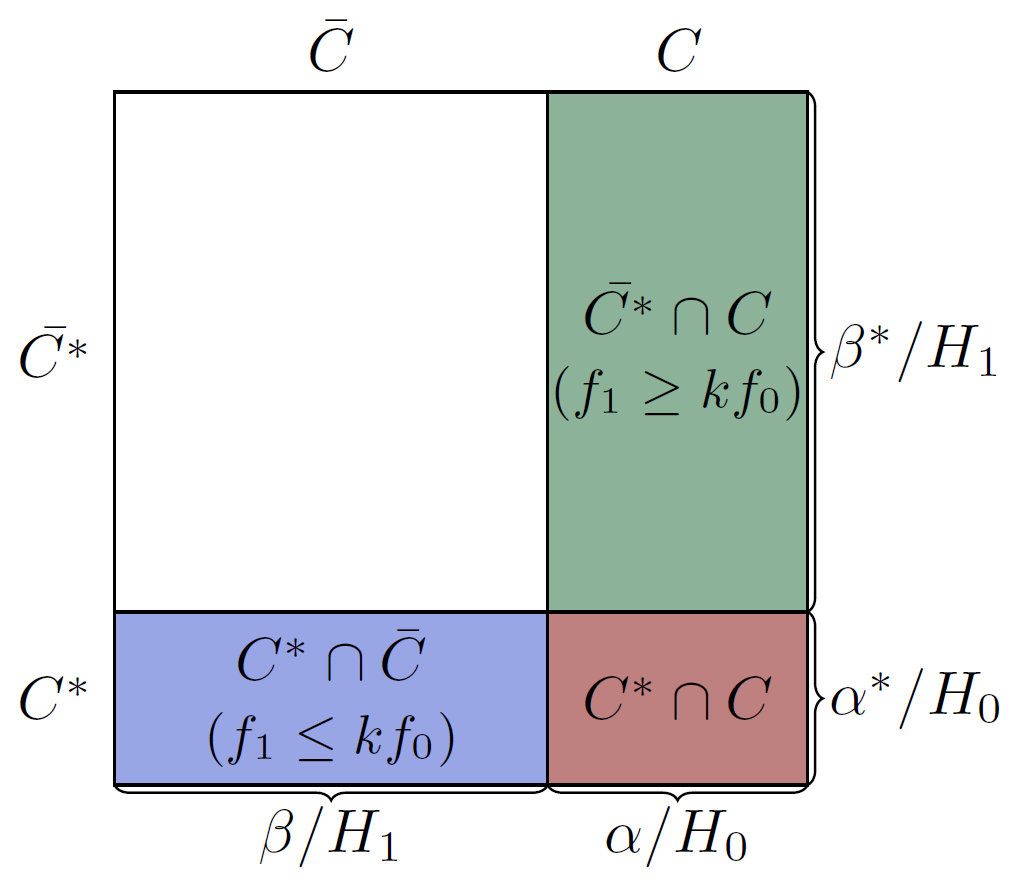
\includegraphics[width=0.45\textwidth]{critregions.PNG}
\end{figure}

Now let $C^*$ be critical region of any other test with size less than or equal to $\alpha$. Let $\alpha^*=\mathbb{P}(\mathbf{X}\in C^*|f_0)$ and $B^*=\mathbb{P}(\mathbf{X}\not\in C^*|f_1)$. We want to show that $\beta\leq\beta^*$.

Now we know that $\alpha^*\leq\alpha$, i.e.
\[
\int_{C^*}f_0(\mathbf{x})d\mathbf{x}\leq\int_Cf_0(\mathbf{x})d\mathbf{x}\,.
\]
On $C$, we have $f_1(\mathbf{x})>kf_0(\mathbf{x})$, while on $\bar{C}$ we have $f_1(\mathbf{x})\leq kf_0(\mathbf{x})$. So
\begin{align*}
    \int_{\bar{C}^*\cap C}f_1(\mathbf{x})d\mathbf{x}&\geq k\int_{\bar{C}^*\cap C}f_0(\mathbf{x})d\mathbf{x}\,,\\
    \int_{\bar{C}\cap C^*}f_1(\mathbf{x})d\mathbf{x}&\leq k\int_{\bar{C}\cap C^*} f_0(\mathbf{x})d\mathbf{x}\,,
\end{align*}
and hence
\begin{align*}
    \beta-\beta*&=\int_{\bar{C}}f_1(\mathbf{x})d\mathbf{x}-\int_{\bar{C}^*}f_1(\mathbf{x})d\mathbf{x}\\
    &=\int_{\bar{C}\cap C^*}f_1(\mathbf{x})d\mathbf{x} + \int_{\bar{C}\cap \bar{C}^*}f_1(\mathbf{x})d\mathbf{x}\\
    &\qquad-\int_{\bar{C}^*\cap C}f_1(\mathbf{x})d\mathbf{x}-\int_{\bar{C}\cap\bar{C}^*}f_1(\mathbf{x})d\mathbf{x}\\
    &=\int_{\bar{C}\cap C^*}f_1(\mathbf{x})d\mathbf{x}-\int_{\bar{C}^*\cap C}f_1(\mathbf{x})d\mathbf{x}\\
    &\leq k\int_{\bar{C}\cap C^*}f_0(\mathbf{x})d\mathbf{x}-k\int_{\bar{C}^*\cap C}f_0(\mathbf{x})d\mathbf{x}\\
    &=k\left\{\int_{\bar{C}\cap C^*}f_0(\mathbf{x})d\mathbf{x}+\int_{C\cap C^*}f_0(\mathbf{x})d\mathbf{x}\right\}\\
    &\qquad-k\left\{\int_{\bar{C}^*\cap C}f_0(\mathbf{x})d\mathbf{x}+\int_{C\cap C^*}f_0(\mathbf{x})d\mathbf{x}\right\}\\
    &=k(\alpha^*-\alpha)\\
    &\leq0\,.
\end{align*}
\end{proof}

Here we assumed that $f_0$, $f_1$ are continuous densities. This is needed to ensure that the likelihood ratio test of exactly size $\alpha$ exists, though even with non-continuous distributions, the likelihood ratio test is still a good idea. In fact, for a discrete distribution, as long as a likelihood ratio test of exactly size $\alpha$ exits, the same result holds.

\begin{ex}
Suppose $X_1,...,X_n$ are i.i.d. $N(\mu,\sigma_0^2)$, where $\sigma_0^2$ is known. We want to find the best size $\alpha$ test of $H_0:\mu=\mu_0$ against $H_1:\mu=\mu_1$, where $\mu_0$ and $\mu_1$ are known fixed values with $\mu_1>\mu_0$. Then
\begin{align*}
    \Lambda_\mathbf{x}(H_0;H_1)&=\frac{(2\pi\sigma_0^2)^{-n/2}\exp\left(-\frac{1}{2\sigma_0^2}\sum(x_i-\mu_1)^2\right)}{(2\pi\sigma_0^2)^{-n/2}\exp\left(-\frac{1}{2\sigma_0^2}\sum(x_i-\mu_0)^2\right)}\\
    &=\exp\left(\frac{\mu_1-\mu_0}{\sigma_0^2}n\bar{x}+\frac{n(\mu_0^2-\mu_1^2)}{2\sigma_0^2}\right)\,.
\end{align*}
This is an increasing function of $\bar{x}$, so for any $k$, $\Lambda_x>k\Leftrightarrow\bar{x}>c$ for some $c$. Hence we reject $H_0$ if $\bar{x}>c$, where $c$ is chosen s.t. $\mathbb{P}(\bar{X}>c|H_0)=\alpha$.

Under $H_0$, $\bar{X}\sim N(\mu_0,\sigma_0^2/n)$, so $Z=\sqrt{n}(\bar{X}-\mu_0)/\sigma_0\sim N(0,1)$. Since $\bar{x}>c\Leftrightarrow z>c'$ for some $c'$, the size $\alpha$ test rejects $H_0$ if 
\[
z=\frac{\sqrt{n}(\bar{x}-\mu_0)}{\sigma_0}>z_\alpha\,.
\]
For example, suppose $\mu_0=5$, $\mu_1=6$, $\sigma_0=1$, $\alpha=0.05$, $n=4$ and $\mathbf{x}=(5.1,5.5,4.9,5.3)$. So $\bar{x}=5.2$.

From the tables, $z_{0.05}=1.645$. We have $z=0.4<1.645$ so $\mathbf{x}$ is not in the rejection region. Thus we do not reject $H_0$ at the 5\%  level and we say that the data are consistent with $H_0$.

Note that this does not mean that we \emph{accept} $H_0$. While we do not have sufficient reason to believe it is false, we also do not have sufficient reason to believe it is true.

This is called a \emph{z-test}.
\end{ex}

In the above example, LR tests reject $H_0$ if $z>k$ for some constant $k$. The size of such a test is $\alpha=\mathbb{P}(Z>k|H_0)=1-\Phi(k)$, and is decreasing as $k$ is increasing. Our observed value $z$ will be in the rejected region iff $z>k\Leftrightarrow\alpha>p^*=\mathbb{P}(Z>z|H_0)$.

\begin{defn}[$p$-value]
The quantity $p^*$ is called the \emph{p-value} of our observed data $\mathbf{x}$. For the example above, $z=0.4$ and so $p^*=1-\Phi(0.4)=0.3446$.
\end{defn}

In general, the $p$-value is sometimes called the ``observed significance level" of $\mathbf{x}$. This is the probability under $H_0$ of seeing data that is ``more extreme" than our observed data $\mathbf{x}$. Extreme observations are viewed as providing evidence against $H_0$.

\subsection{Composite hypotheses}
For composite hypotheses like $H:\theta\geq0$, the error probabilities do not have a single value. We define

\begin{defn}[Power function]
The \emph{power function} is
\[
W(\theta)=\mathbb{P}(\mathbf{X}\in C|\theta)=\mathbb{P}(\text{reject }H_0|\theta)\,.
\]
We want $W(\theta)$ to be small on $H_0$ and large on $H_1$.
\end{defn}

\begin{defn}
The \emph{size} of the test is
\[
\alpha=\sup_{\theta\in\Theta_0}W(\theta)\,.
\]
\end{defn}

This is the worst possible size we can get.

For $\theta\in\Theta_1$, $1-W(\theta)=\mathbb{P}(\text{Type II error}|\theta)$.

Sometimes the Neyman-Pearson theory can be extended to one-sided alternatives. For example, in the previous example, we have shown that the most powerful size $\alpha$ of $H_0:\mu=\mu_0$ versus $H_1:\mu=\mu_1$ (where $\mu_1>\mu_0$) is given by 
\[
C=\left\{x:\frac{\sqrt{n}(\bar{x}-\mu_0)}{\sigma_0}>z_\alpha\right\}\,.
\]
This critical region depends on $\mu_0,n,\sigma_0,\alpha$, and the fact that $\mu_1>\mu_0$. It does not depend on the particular value of $\mu_1$. This test is then uniformly the most powerful size $\alpha$ test for testing $H_0:\mu=\mu_0$ against $H_1:\mu>\mu_0$.

\begin{defn}
A test specified by a critical region $C$ is \emph{uniformly most powerful} (UMP) size $\alpha$ test for testing $H_0:\theta\in\Theta_0$ against $H_1:\theta\in\Theta_1$ if
\begin{enumerate}
    \item $\sup_{\theta\in\Theta_0}W(\theta)=\alpha$.
    \item For any other test $C^*$ with size $\leq\alpha$ and power function $W^*$, we have $W(\theta)\geq W^*(\theta)\;\forall\theta\in\Theta_1$.
\end{enumerate}
Note that these may not exist, but the likelihood ratio test often works.
\end{defn}

\begin{ex}
Suppose $X_1,...,X_n$ are i.i.d. with $N(\mu,\sigma_0^2)$ where $\sigma_0$ is known, and we wish to test $H_0:\mu\leq\mu_0$ against $H_1:\mu>\mu_0$.

First consider testing $H_0':\mu=\mu_0$ against $H_1':\mu=\mu_1$, where $\mu_1>\mu_0$. The Neyman-Pearson test of size $\alpha$ of $H_0'$ against $H_1'$ has
\[
C=\left\{x:\frac{\sqrt{n}(\bar{x}-\mu_0)}{\sigma_0}>z_\alpha\right\}\,.
\]
We show that $C$ is in fact UMP for the composite hypotheses $H_0$ against $H_1$. For $\mu\in\mathbb{R}$, the power function is 
\begin{align*}
    W(\mu)&=\mathbb{P}_\mu(\text{reject }H_0)\\
    &=\mathbb{P}_\mu\left(\frac{\sqrt{n}(\bar{x}-\mu_0)}{\sigma_0}>z_\alpha\right)\\
    &=\mathbb{P}_\mu\left(\frac{\sqrt{n}(\bar{x}-\mu)}{\sigma_0}>z_\alpha+\frac{\sqrt{n}(\mu_0-\mu)}{\sigma_0}\right)\\
    &=1-\Phi\left(z_\alpha+\frac{\sqrt{n}(\mu_0-\mu)}{\sigma_0}\right)\,.
\end{align*}
Now from direct evaluation, $W(\mu_0)=\alpha$, and $W(\mu)$ is an increasing function of $\mu$. So $\sup_{\mu\leq\mu_0}W(\mu)=\alpha$.

For the second condition, observe that for any $\mu>\mu_0$, the Neyman-Pearson size $\alpha$ test of $H_0'$ vs $H_1'$ has critical region $C$. Let $C^*$  and $W^*$ belong to any other test of $H_0$ vs $H_1$ of size $\leq\alpha$. Then $C^*$ can be regarded as a test of $H_0'$ vs $H_1'$ of size $\leq\alpha$, and the Neyman-Pearson lemma says that $W^*(\mu_1)\leq W(\mu_1)$. This holds for all $\mu_1>\mu_0$. So the condition is satisfied and the test is UMP.
\end{ex}

\begin{defn}[Likelihood of composite hypothesis]
The \emph{likelihood} of a composite hypothesis $H:\theta\in\Theta$ given data $\mathbf{x}$ is
\[
L_\mathbf{x}(H)=\sup_{\theta\in\Theta}f(\mathbf{x}|\theta)\,.
\]
\end{defn}

So far we have taken disjoint hypotheses $\Theta_0,\Theta_1$, but we may not be interested in any specific alternative. So we can instead take $\Theta_1=\Theta$ rather than $\Theta\setminus\Theta_0$. Then
\[
\Lambda_\mathbf{x}(H_0;H_1)=\frac{L_\mathbf{x}(H_1)}{L_\mathbf{x}(H_0)}=\frac{\sup_{\theta\in\Theta_1} f(\mathbf{x}|\theta)}{\sup_{\theta\in\Theta_0} f(\mathbf{x}|\theta)}\geq 1\,,
\]
with large values of $\Lambda$ indicating departure from $H_0$.


\end{document}
